\documentclass[10pt,pdf,hyperref={unicode}, dvipsnames]{beamer}
\usepackage[english,russian]{babel}
% \usepackage[T2A,T1]{fontenc}
\usepackage[utf8]{inputenc}
\usepackage{tikz}
\usepackage[unicode]{hyperref}
\usepackage{pgfplots,standalone}
% \usepackage{lmodern}
\pgfplotsset{compat=newest} 
\usetikzlibrary{%
    decorations.pathreplacing,%
    decorations.pathmorphing,%
    patterns,%
    angles,%
    quotes,%
    calc, %
    3d, %
    backgrounds, %
    positioning%
}

% Стиль презентации
\usetheme{Warsaw}

% \setbeamercolor{frametitle right}{fg=white,bg=Brown!85}
% \setbeamercolor{frametitle}{fg=white,bg=Brown!85}
\setbeamercolor{frametitle right}{fg=white,bg=black!85}
\setbeamercolor{frametitle}{fg=white,bg=black!85}

\setbeamertemplate{headline}{}
\setbeamertemplate{footline}{}
\let\Tiny=\tiny % решает проблему со шрифтами в TexLive
\setbeamertemplate
	{footline}{
		\color{black!40!white}
		\quad\hfill
		\insertframenumber/\inserttotalframenumber
		\hfill\vspace{1em}\quad
	} 

\setbeamertemplate{navigation symbols}{}

\beamersetrightmargin{0.5cm} 
\beamersetleftmargin{0.5cm}

\setbeamertemplate{enumerate item}{
	\usebeamercolor[bg]{item projected}
	\raisebox{1pt}{\colorbox{bg}{\color{fg}\footnotesize\bf\insertenumlabel}}%
}
\setbeamercolor{item projected}{bg=black,fg=white}

\setbeamertemplate{itemize item}{%
	\usebeamercolor[bg]{item projected}%
	\raisebox{1pt}{{\color{bg}\footnotesize$\bf\square$}}%
}
\setbeamercolor{item projected}{bg=black,fg=white}
\setbeamercolor{title}{bg=black,fg=white}
\newcommand\frametitless[1]{\subsection{#1}\frametitle{#1}}
\usepackage{booktabs, setspace}
\newcommand{\tabitem}{~~\llap{\textbullet}~~}
\setbeamertemplate{caption}{\raggedright\insertcaption\par}
\title[]{Изучение электромагнитных резонансных явлений в резонаторе Земля--ионосфера}

\author{%
	Сарафанов Ф.Г., %
	Платонова М.В. %
}

\institute{Радиофизический факультет ННГУ, 420 группа}

\date{Нижний Новгород, 2017}

\begin{document}  

%%%%%%%%%%%%%%%%%%%%%%%%%%%%%%%%%%%%%%%%%%%%%%%%%%%%%%%%%%%%%
\begin{frame}[plain]
	\centering
	\vspace{2cm}
	\begin{beamercolorbox}[sep=8pt,center]{title}
		\bf\usebeamerfont{title}\inserttitle
	\end{beamercolorbox}
	\vspace{0.5cm}
	\normalsize \textbf{Работу выполнили:}\\
	\large\insertauthor\\ 
	\vspace{0.5cm}
	\normalsize{\textbf{Научные руководители:}\\}
	\large{Мареев Е.А., Шлюгаев Ю.В.}
	\vfill
	\small{Нижний Новгород -- 2018}
\end{frame}
%%%%%%%%%%%%%%%%%%%%%%%%%%%%%%%%%%%%%%%%%%%%%%%%%%%%%%%%%%%%%
% \begin{frame}[t]
%   \frametitle{Содержание}
%   \tableofcontents
% \end{frame}
%%%%%%%%%%%%%%%%%%%%%%%%%%%%%%%%%%%%%%%%%%%%%%%%%%%%%%%%%%%%%
\section{Цели работы}
\begin{frame}[t]
	\frametitle{Цели работы}
	% \textbf{Цели}\\
	\vfill
\begin{spacing}{1}
	\begin{enumerate}
		\item Изучить явление резонанса в резонаторе Земля-ионосфера
		\item Создать программу обработки данных для определения резонансных частот
		\item Обработать экспериментальные данные и объяснить характерные особенности спектрограммы  
		\item Определить направление на источники сигнала, выявленные на спектрограмме
	\end{enumerate}
\end{spacing}
	\vfill
\end{frame}
%%%%%%%%%%%%%%%%%%%%%%%%%%%%%%%%%%%%%%%%%%%%%%%%%%%%%%%%%%%%%
\section{Теоретическая часть}
\begin{frame}[t]
	\frametitless{Глобальная электрическая цепь}
	% \begin{enumerate}
		% \item \textbf{Спонтанное излучение}
	% \end{enumerate}
	\vspace{-1em}
	\begin{center}
		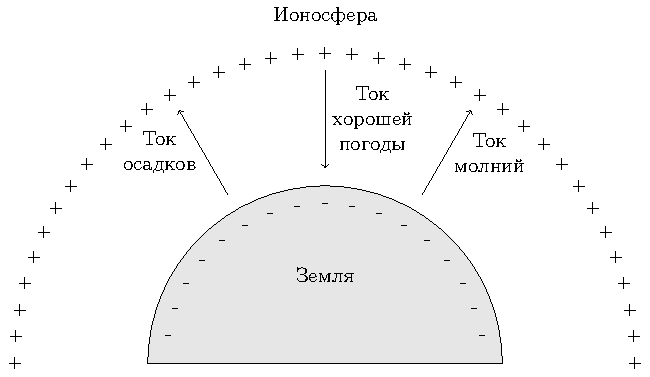
\includegraphics[width=0.9\textwidth]{images/spont}
	\end{center}
	Разность потенциалов между Землей и ионосферой составляет $\approx 300$ кВ

	Основная зарядка происходит в мировых грозовых центрах: дельта Амазонки (Южно-американский грозовой центр), дельта реки Конго (Африканский грозовой центр).
\end{frame}
%%%%%%%%%%%%%%%%%%%%%%%%%%%%%%%%%%%%%%%%%%%%%%%%%%%%%%%%%%%%%
\begin{frame}[t]
	\frametitless{Возникновение резонанса в сферическом резонаторе Земля-ионосфера}
	\vfill
	\begin{columns}
		\begin{column}{0.49\textwidth}
			Возникшая в резонаторе ЭМ-волна после огибания земного шара и ряда отражений может войти в резонанс с собой. 
			\vspace{1em}

			% В грубом приближении, это может произойти при целом количестве отражений границы Земли и ионосферы (при условии идеального отражения и не учитывая эффекты, связанные с отражением от границы раздела двух сред) 
			Такой резонанс возможен на частотах
			\begin{equation*}
			 	f=\frac{cn}{2\pi R},
			\end{equation*} 
			гдe $n$ -- число отражений, $c$ -- скорость волны, $R$ -- радиус Земли
			\vspace{1em}

			Это явление \textbf{шумановского резонанса}.
	
		\end{column}
		\begin{column}{0.49\textwidth}
			\begin{figure}[h]
				\centering
				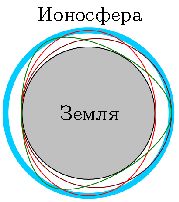
\includegraphics[scale=1.5]{images/sh}
				% \caption{Возникновение устойчивых мод}
			\end{figure}	
		\end{column}
	\end{columns}	
	\vfill
\end{frame}
%%%%%%%%%%%%%%%%%%%%%%%%%%%%%%%%%%%%%%%%%%%%%%%%%%%%%%%%%%%%%
\begin{frame}[t] 
	\frametitless{Характерный вид резонансных пиков шумановских частот}
	\begin{figure}[h]
		\centering
		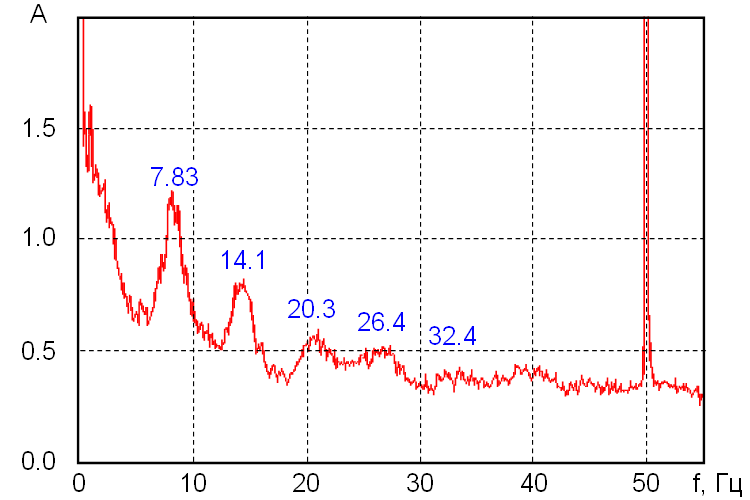
\includegraphics[width=0.7\textwidth]{images/sp.png}
				\caption{Спектрограмма [из интернета] измерений магнитного поля}
	\end{figure}	
\end{frame}

% %%%%%%%%%%%%%%%%%%%%%%%%%%%%%%%%%%%%%%%%%%%%%%%%%%%%%%%%%%%%%
\begin{frame}[t]
	\frametitless{Аппаратура}
	Данные, обрабатываемые в данной работе, получены при помощи двух разнесенных с базой $l=50$ м установок, каждая из которых представляет три взаимно перпендикулярных индукционных датчика IMS-008.

	\begin{columns}
		\begin{column}{0.49\textwidth}
			\begin{figure}[h]
				\centering
				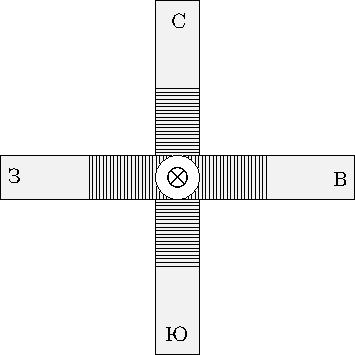
\includegraphics[scale=0.8]
				{images/us}
			\end{figure}	
		\end{column}
		\begin{column}{0.49\textwidth}

			Наличие в месте измерений сильной помехи на частоте сети 50 Гц и ее гармоник до 500 Гц обусловило выбор частоты дискретизации

			\begin{equation*}
				f_d=2000 \text{ Гц },
			\end{equation*}

			которая заведомо больше частоты Найквиста.

			\vspace{1em}
			Разрешение АЦП позволяет измерять частоты от 0.1 Гц до 10 кГц.
		\end{column}
	\end{columns}
	\vspace{1em}
	Точка измерения магнитного поля -- 69.2517N, 35.1561E (Териберский маяк, Териберка, Кольский полуостров).

\end{frame}
% %%%%%%%%%%%%%%%%%%%%%%%%%%%%%%%%%%%%%%%%%%%%%%%%%%%%%%%%%%%%%
\begin{frame}[t]
	\frametitless{Обработка данных. Дискретное преобразование Фурье}
	\vspace{-0.5em}

	\begin{enumerate}
		\item $H(t) \Rightarrow H(f)$
		\item Дискретное преобразование Фурье
		\item Быстрое преобразование Фурье (1 час сигнала - 40 минут преобразование)
	\end{enumerate}
	% Интерес для исследования представляет не снятая зависимость $H(t)$, а ее спектральное представление, полученное дискретным преобразованием Фурье (ДПФ):
	\vspace{-0.8em}
	\begin{figure}[h]
		\centering
		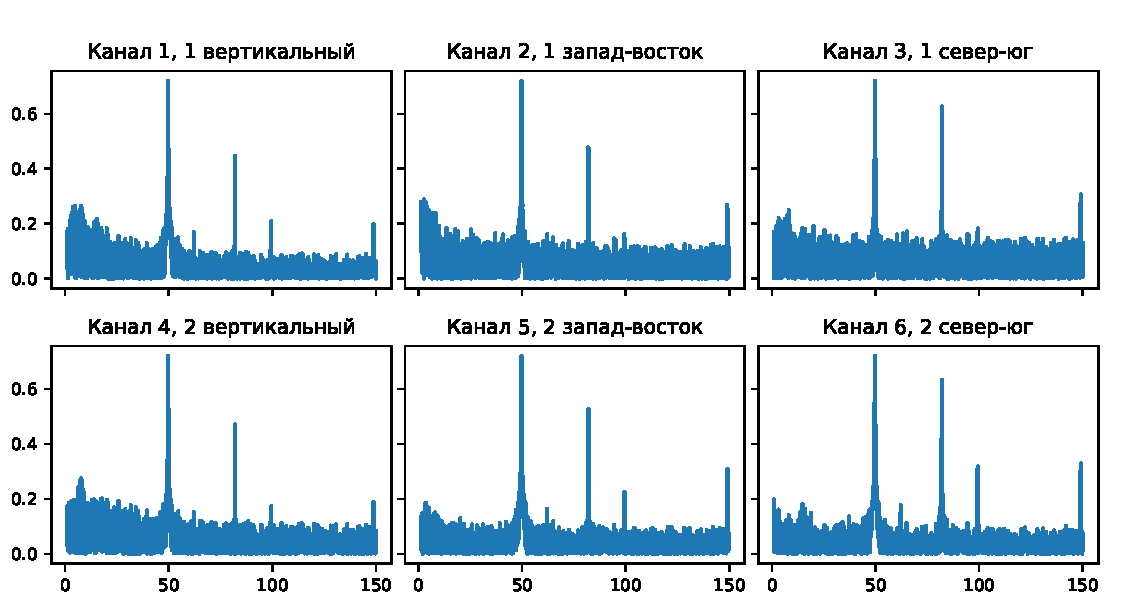
\includegraphics[width=1\textwidth]{images/6g.pdf}
		% \caption{4-уровневая среда}
	\end{figure}	


\end{frame}
% %%%%%%%%%%%%%%%%%%%%%%%%%%%%%%%%%%%%%%%%%%%%%%%%%%%%%%%%%%%%%
\begin{frame}[t]
	\frametitless{Фильтрация данных}
	\begin{enumerate}
		\item Децимация данных, фильтрация фильтром Баттерворта 3-го порядка. ФНЧ ($f_c=150$ Гц), ФВЧ ($f_c=0.2$ Гц)
		\item Децимация спектра и усреднение полосами шириной 2 Гц
		% \item Быстрое преобразование Фурье (1 час сигнала - 40 минут преобразование)
	\end{enumerate}
	% Для возможности анализировать низкие частоты в спектре данные обработаны двумя электронным фильтрами -- ФНЧ и ФВЧ Баттерворта 3-го порядка, далее децимированы и усреднены полосами шириной 2 Гц:
	% \vspace{-1em}
	\begin{figure}[h]
		\centering
		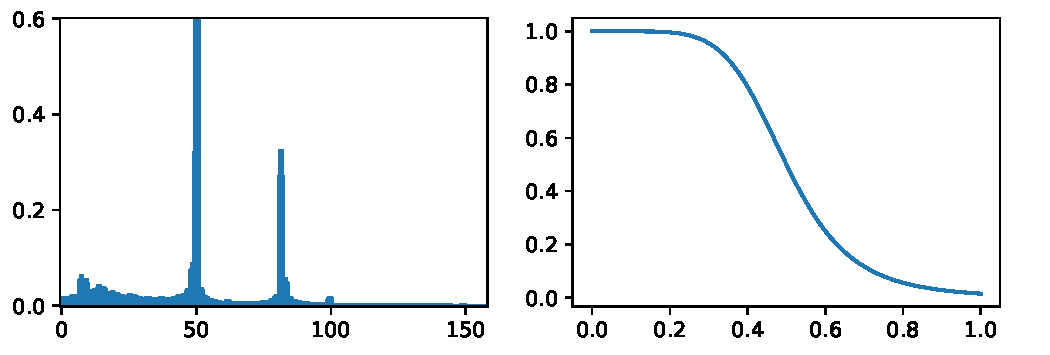
\includegraphics[width=1\textwidth]{images/bt2.pdf}
		\caption{Отфильтрованные данные и АЧХ фильтра Баттерворта}
	\end{figure}	
\end{frame}
% %%%%%%%%%%%%%%%%%%%%%%%%%%%%%%%%%%%%%%%%%%%%%%%%%%%%%%%%%%%%%
\begin{frame}[t]
	\frametitless{Резонансные частоты Шумана}
	\begin{enumerate}
		\item Выделен спектр шумановских резонансных частот -- 8, 14, 20, 26, 32 Гц
		\item Спектр ниже 8 Гц потерян, но в данной работе не используется
		% \item Быстрое преобразование Фурье (1 час сигнала - 40 минут преобразование)
	\end{enumerate}
	% После обработки стали доступны для наблюдения гармоники шумановского резонанса, примерно 8 и 14 герц и следующие:
	% \vspace{-1em}
	\begin{figure}[h]
		\centering
		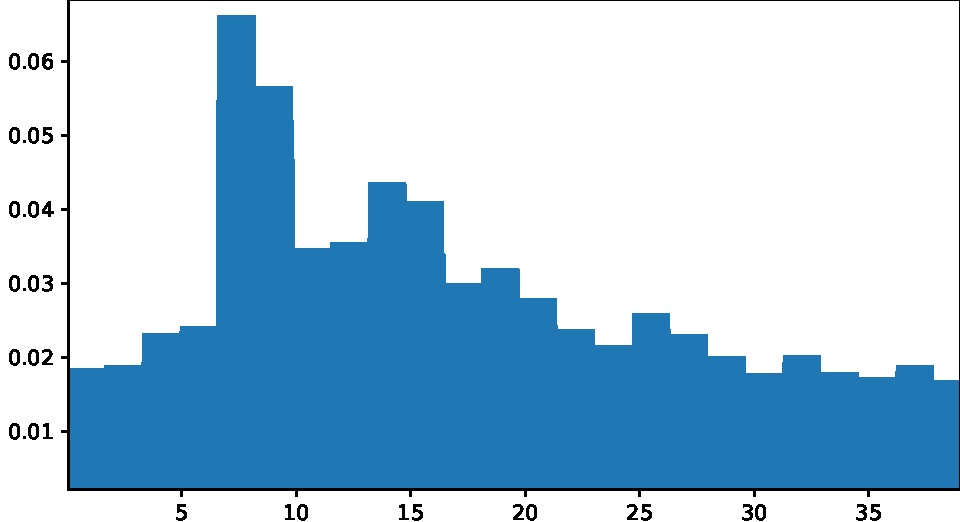
\includegraphics[width=0.8\textwidth]{images/12.pdf}
		\caption{Первые гармоники шумановского резонанса}
	\end{figure}	
\end{frame}
% %%%%%%%%%%%%%%%%%%%%%%%%%%%%%%%%%%%%%%%%%%%%%%%%%%%%%%%%%%%%%
\begin{frame}[c]
	\frametitless{Направления на источники. Сравнение амплитуд}
	Простейший способ определения направления на источник заключался в сравнении амплитуд $H_{\text{зв}}$ и $H_{\text{cю}}$ резонансных пиков:
	\begin{equation*}
		\alpha=\arctan{\frac{H_{\text{зв}}}{H_{\text{cю}}}}
	\end{equation*}
	\begin{enumerate}
		\item Направление на генератор 50 Гц, рассчитанное таким способом, $\approx43^\circ$. Реальное направление на источник -- $45^\circ$
		\item Найдено направление на источник шумановского резонанса $\approx15^\circ$. Реальное направление на источник -- $\approx 5^\circ$
		\item Направление на станцию радиосвязи <<Зевс>> (82Гц) $\approx54^\circ$. Реальное направление на источник  $\approx60^\circ$
		% \item Быстрое преобразование Фурье (1 час сигнала - 40 минут преобразование)
	\end{enumerate}
\end{frame}
\begin{frame}
	\frametitless{Выводы}
	\begin{enumerate}
		\item Исследована природа резонанса Шумана
		\item Изучено применение методов определения местоположения грозовой активности
		\item Написана программа для обработки экспериментальных данных, с помощью нее получены спектрограммы магнитного поля
		\item Проведен анализ спектрограмм, на которых выделялись:
		\begin{enumerate}
		 \item Пять гармоник резонансных частот Шумана (8 Гц, 14 Гц, 20 Гц, 26 Гц, 32 Гц)
		 \item сеть с частотой 50 Гц и ее гармоники
		 \item сеть станции СДВ-радиосвязи  <<Зевс>>
		  \end{enumerate}
		\item Определены направления на шумановский резонанс ($\approx15^\circ$), генератор ($\approx43^\circ$ ), станцию радиосвязи <<Зевс>> ($\approx52^\circ$) 
	\end{enumerate}
\end{frame}

%%%%%%%%%%%%%%%%%%%%%%%%%%%%%%%%%%%%%%%%%%%%%%%%%%%%%%%%%%

\begin{frame}[plain]
	\vspace{4cm}
	\begin{center}
		\Huge
		Спасибо за внимание!
	\end{center}
	\vspace{2.5cm}
	\begin{center}
		\color{black!70!white}
		Презентация подготовлена в издательской \\
		системе LaTeX с использованием пакетов \\
		PGF/TikZ и Beamer
	\end{center}
\end{frame}


\end{document}